% NOTE - this is only a template without real arguments
\begin{entry}{Example Title}{Dec 01, 2020}
    \objective 
    
    What do you want to do?
    
    \outline
    
    What steps are required?
    
    \procedures
    
    How do you do each step?
    
    \parameters
    
    What are the key elements of the objective?
    
    \observations
    
    What happened?
    
    \data
    
    All recorded data, or where it can be found.
    
    \results
    
    Did you achieve your objective?
    
\end{entry}


\begin{entry}{CMake Error running EGOT-DCM Dockerfile}{Dec 02, 2020}
    \objective 
    
    Determine the cause of the CMake error while running the dockerfile and modify file to get it to successfully build.
    
    \outline
    
    \begin{itemize}
        \item Try running to see if it was just Lorry or a machine issue.
        \item If it is a machine issue, modify configurations to ensure interoperability.
        \item If I get the error track down its cause and modify dockerfile to fix.
        \item Repeat until all builds are successful.
    \end{itemize}
    
    \procedures
    
    \begin{itemize}
        \item \mint{console}|git clone https://github.com/EGoT-DCS-SunSpec-Modbus|
        \item \mint{console}|docker build -f Dockerfile.buster -t egot-dcs .|
        \item \mint{console}|docker container run -i egot-dcs|
    \end{itemize}
    
    \observations

    \begin{error}{Cmake Error: No CMAKE\_CXX\_COMPILER found}
        \begin{figure}[H]
            \centering
            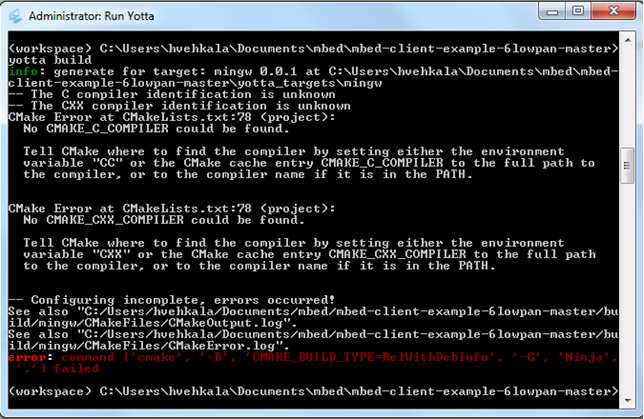
\includegraphics[height=4in]{Fall2020/Figures/cmake_error.png}
        \end{figure}
        
        Solution: what you need to do found at \cite{CMAKE-Forum}
    \end{error}
    
    \results
    
    Short: No.
    
    Long: Well...
    

\end{entry}